\documentclass[letterpaper]{article}
\usepackage{amssymb}
\usepackage{fullpage}
\usepackage{changepage}
\usepackage{amsmath}
\usepackage{epsfig,float,alltt}
\usepackage{psfrag,xr}
\usepackage[T1]{fontenc}
\usepackage{url}
\usepackage{pdfpages}
\usepackage{epstopdf}
\usepackage[framed,numbered,autolinebreaks,useliterate]{mcode}

%\includepdfset{pagecommand=\thispagestyle{fancy}}
\author{Fan Bu, Feng Zhou, Yi Yang}
\title{ME 552 Lab 01 Report}

\begin{document}
\date{09/17/2016}
\maketitle

\newcommand{\trace}{\mathrm{trace}}
\newcommand{\real}{\mathbb R}  % real numbers  {I\!\!R}
\newcommand{\nat}{\mathbb N}   % Natural numbers {I\!\!N}
\newcommand{\cp}{\mathbb C}    % complex numbers  {I\!\!\!\!C}
\newcommand{\ds}{\displaystyle}
\newcommand{\mf}[2]{\frac{\ds #1}{\ds #2}}
\newcommand{\spanof}[1]{\textrm{span} \{ #1 \}}
\newcommand{\sol}[0]{\textbf{Solution: }}
\newcommand{\pf}[0]{\textbf{Proof:}}
\newcommand{\rme}[0]{\textrm{e}}
\newcommand{\Null}[1]{\textrm{Null}\{#1\}}
\parindent 0pt
%%%%%%%%%%%%%%%%%%%%%%%%%%%%%%%%%%%%%%%%%%%%%%%%%%%%%%%%%%%%%%%%%%%%%%%%%%%%%%%
% Solution for Question 1 begins here - by Yi Yang
%%%%%%%%%%%%%%%%%%%%%%%%%%%%%%%%%%%%%%%%%%%%%%%%%%%%%%%%%%%%%%%%%%%%%%%%%%%%%%%
\section*{Question 1}
\subsection*{(a)}
We design the circuit as shown below:\\
\begin{figure}[h]
\begin{center}
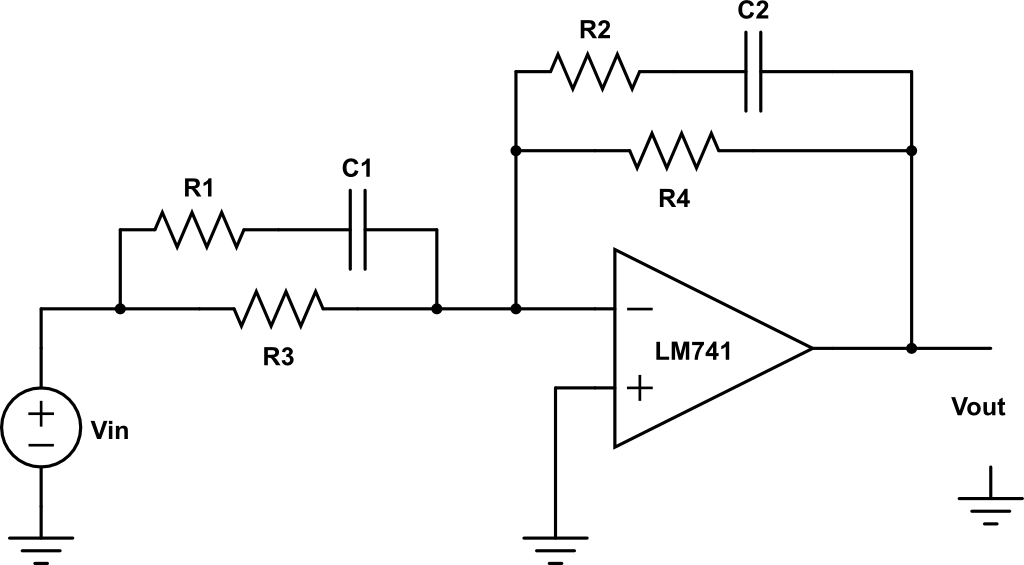
\includegraphics[width=10cm]{q1_circuitDiagram.png}
\end{center}
\caption{A lead-lag compensator circuit diagram for question 1.}
\label{q1_a}
\end{figure}
\subsection*{(b)}
We can let $R_1$, $C_1$, $R_3$ and $R_2$, $C_2$, $R_4$ form two different impedance module separately, and let their impedance equal $Z_1$ and $Z_2$, we can get:
$$Z_1 = \frac{R_3 * (R_1 + (1/sC_1))}{R_3 + (R_1 + (1/sC_1))} = \frac{R_3(sR_1C_1 +1)}{s(R_1C_1 + R_3C_1) + 1}$$
$$Z_2 = \frac{R_4 * (R_2 + (1/sC_2))}{R_4 + (R_2 + (1/sC_2))} = \frac{R_4(sR_2C_2 +1)}{s(R_2C_2 + R_4C_2) + 1}$$
The new circuits can be seen as an inverting amplifier:
$$\frac{V_{out}(s)}{V_{in}(s)} = - \frac{Z_2}{Z_1} = -  \frac{R_4(sR_2C_2 +1)}{(s(R_2C_2 + R_4C_2) + 1)}\frac{(s(R_1C_1 + R_3C_1) + 1)}{R_3(sR_1C_1 +1)} $$
$$=  -  \frac{R_4}{R_3}\frac{(sR_2C_2 +1)}{(s(R_2C_2 + R_4C_2) + 1)}\frac{(s(R_1C_1 + R_3C_1) + 1)}{(sR_1C_1 +1)} $$
If we assume $R_3 = R_4$, we will gain the standard formula of lead-lag compensator.
\end{document}